\documentclass[Journal, BackFigs, DoubleSpace]{ascelike} %NewProceedings, Journal

%include package for inserting picture
\usepackage{graphicx}%insert image
\DeclareGraphicsExtensions{.pdf,.png,.jpg}
\graphicspath{{figures/}}%folder contains images

\usepackage{caption}%packages for inserting multiple pictures
\usepackage{subcaption}%packages for inserting multiple pictures

\usepackage{array}%for table with fixed width
\newcolumntype{L}[1]{>{\raggedright\let\newline\\\arraybackslash\hspace{0pt}}m{#1}}
\newcolumntype{C}[1]{>{\centering\let\newline\\\arraybackslash\hspace{0pt}}m{#1}}
\newcolumntype{R}[1]{>{\raggedleft\let\newline\\\arraybackslash\hspace{0pt}}m{#1}}

\usepackage{amsmath} %math package

\usepackage{algorithm} %algorithm package
\usepackage[noend]{algpseudocode} % pseudo code package

\usepackage[utf8]{inputenc}%french accents
\usepackage[T1]{fontenc} %for accented characters

\usepackage{booktabs}%allowing drawing hline in table crossing only some columns

\usepackage{enumitem}


\begin{document}

\title{InfraLex: A digital dictionary for unambiguous data sharing \\in the civil infrastructure domain}
%TODO: distinguish between lexicon, thesaurus and ontology
%
\author{
Tuyen Le
\thanks{
Ph.D. Candidate, Department of Civil, Construction and Environmental Engineering, Iowa State University. Ames, IA 50011, United States. E-mail: ttle@iastate.edu.},
\and
H. David Jeong
\thanks{Associate Professor, Department of Civil, Construction and Environmental Engineering, Iowa State University. Ames, IA 50011, United States. E-mail: djeong@iastate.edu.}
 }

\maketitle
%
%\begin{center}
%(To be submitted to the Journal of Computing in Civil Engineering) 
%\end{center}

\begin{abstract} %150-175 words (as required by ASCE)
%background:
The inconsistency of data terminology due to the fragmented nature of the civil infrastructure industry has imposed big challenges on integrating digital data from distinct sources to support decision making in asset management. The issue of data ambiguity may lead to a lack of common understanding to the same data between the sender and receiver. While the heterogeneity of data formats has been well addressed thanks to the availability of various international neutral data standards such as LandXML and TransXML;  the semantic aspect still has been neglected by the domain researchers. 
%research objective
This paper presents a novel methodology to construct an automatically-generated lexicon, namely InfraLex, that formally organizes civil infrastructure technical terms in a lexical hierarchy manner. The lexicon severs as a digital dictionary of domain terms which would enable data integration systems to understand the meaning of a data representation, and helps avoid the mismatch of data.
%research methods
Natural Language Processing (NLP) techniques and the C-value method are used to detect technical terms from a highway text corpus collected from roadway design guidelines across the State Departments of Transportation. A model for measuring term similarity is trained using the Skip-gram model which uses the corpus as the training dataset. This semantic model is then utilized by a term classification algorithm that organizes related terms into separate groups according to their semantic relations.
%result
The developed lexicon was evaluated by conducting an experiment comparing the automatically-identified synonyms with a human-constructed synonym set. The result shows that the proposed model achieved a precision of over 80 percent.
  
\end{abstract}

\KeyWords{Civil infrastructure project, Lexicon, Data sharing, Semantic interoperability, NLP, Vector space model}
%
%\newpage


%********************************************************
%good terms and phrases:

%adj: nonhierarchical, superior, well-defined; foreseeable; rigid, flexible, empirical, disparate, isolated, labrious and resouce-intensive, proprietary, integrated, shared, inefficent, time-consuming, laborious, prone error, consistent, easy-to-use, intuitive solutions, extensive, transformative impact, labour extensive, 

%sentence strucutre:  this is evidenced by the accelerating emergence of ...; 

%noun: challenges, barrier, hinders, obstacles, impediment; that approximate concepts; extraction=deduction=acquisition; broad spectrum; overtake these technical and economic challenges; bottleneck; data crreation and utilization; in the midst of planning; interpretation; multitude of data,  data repository, a structured system of terms, data representation, initiatives, bottleneck, insight and value from massive amounts of data, technology and skillset, data scale, magnitude,  a plethora of, data sharing pardigm, inconsistency, discrepancy, the origin of, vicinity=neigborhood, very little of st, 

%verb: emcombass; tackle, foster, amplified; simplified; detect; aggregate; encompass, manifest,envision,  is divided into two, is shared among,  derive, extract, eunsure data to be understood, 

%adv: namely, undoubtedly, oftentimes, cohesively, extensively,

%linking: thereby, only those concepts that, whereby, 

%sentence template: tailored with respect to their context; includes three phases, namely AA, BB and CC; at such places as parks, fairgounds or town spuares; case-specific developments; area of interests; incrementally built; inexpensive and easy-to-use testing device; time and cost-efficient way; research community; one of..since then is the; RDF structure..to make assertion about a resource; syntax-centered NLP;  such as A, B, etc.; ..is in it's reliance upon the presence..which is..; with the objectives of disambiguation; has triggered a mounting awareness; to be the main impediment to the progess; ..start point for deducing other truth; lastly; there is a large body of research on; see e.g. [2], [14] and [32]; the former, the latter; rigorously formalized; backbone strucutre of st; was opted to; Sections 4.5 and 4.6; (e.g., Neo4J, OrientDB, Titan); forthcoming year; well-designed process; is subject to do st; in turn means that; discussion by academics and professionals; some insights on planning, management, and control; strategic framework; in-depth project performance; in lieu of; 

%term': empirical work; linguistic unit/term; 

%axiomatic richness, formality of representation,  

%the following expression denotes, is presented/defined as follows, this/below example shows, the snippet below presents, the following is the short description of the rule, an OWL ontology describing an ifcwindow class, these concepts and relationships can be encoded in the following RDF/XML fragment, is written in Turtle syntax/format:
%The tool is meant to assess, 
%********************************************************

\section{Introduction}%900 words
%Topic introduction, territory: centrality--> genearal background information 
%the background of data extraction
%
The implementation of advanced computerized technologies such as 3D modeling and Geographic Information System (GIS) throughout the life cycle of a civil infrastructure project has allowed a large portion of project data to be available in digital format. The efficiency improvement in sharing these data between project participants and stages, will in turn, translate into increased productivity, efficiency in project delivery and accountability. However, a highway asset as a whole has not yet fully benefited from the potentials of digital models as an accessible, reusable and reliable information source for life-cycle decision making due to the interoperability issue. According to a study conducted by the National Institute of Standard and Technology (NIST), the un-interoperability issue was reported to cost the U.S. capital facilities industry at least \$15.8 billion per year, and two-thirds of those costs were incurred during the operation and maintenance stages \cite{Gallaher04}. The major cost was time spent finding, verifying, and transferring facility and project information into a useful format. This finding indicates that the lack of readiness for downstream phases to directly use the transferred digital project data generated from upstream design and construction stages results in high operational costs.
\par
Semantic interoperability, which relates to the issue whereby two computer systems may not have the same understanding to the same piece of data, is a radical barrier to computer-to-computer data exchange. Due to the fragmented nature of the infrastructure domain, data representation/terminology varies between phases, stakeholders, or geographic regions (counties, states, etc.). Retrieving the right pieces of data in such a heterogeneous environment becomes increasingly complex \cite{karimi2003semantic}. Polysemy and synonymy are two major semantic obstacles to the integration and use of a multitude of data sources. Polysemy refers to cases when a unique term has several distinct meanings. For example, the term \textit{roadway type} can either mean \textit{material classification} or \textit{functional classification} of roadways. In contrast, synonymy is associated with the diversity of terms for the same concept. For instance, the longitudinal centerline of a roadway has various terms including `profile', `crest', `grade-line' and `vertical alignment'. Simply mapping of data names will likely lead to the failure of data extraction, or use of wrong data. Thus, addressing the terminology ambiguity issue becomes crucial to ensure the common understanding on the same dataset between software applications and guarantee the extraction of right data and proper integration of data from multiple sources.
\par
%niche: the importance of dictionaries, ontologies to text analysis, mining and the shortage of dictionaries in civil industry
An extensive amount of research effort has been made for the last several decades in standardizing a neutral format for life-cycle data sharing, such as Industry Foundation Classes (IFC) \cite{buildingsmartIFC} and LandXML \cite{landxml15}. However, research to address the issue of terminology inconsistency in the construction industry has been very limited. Filling this gap has been a top aim of the research efforts to realize the seamless exchange of digital data. One of the approaches to enable proper and ambiguity-free reuse of digital data is to develop Model View Definitions (MVDs) \cite{buildingSmart}. MVD formally identifies a mapping matrix between the data entities in a neutral data schema and the domain data labels for a specific transaction scenario. MVD enables partial models to be easily extracted and unambiguously interpreted. However, this approach is on a case-by-case and manual basis, and takes years to be completed and maintained\cite{venugopal12,eastman12}; there is a demand for more rigorous computational techniques that can allow for automated extraction of data with minimized human intervention. A more robust approach to the issue of data inconsistency is to develop a digital dictionary that explains domain concepts in a machine-readable format. A few construction domain specific semantic resources have been proposed; for example, the Civil Engineering Thesaurus (CET) \cite{abuzir02}, e-Cognos \cite{wetherill02}, and buildingSMART data dictionary (ISO 12006-3) \cite{buildingsmartData}. These digital knowledge bases allow computer systems to precisely understand meanings of terms. Thus, data mismatch when unifying isolated data sources would be eliminated. They, however, are mainly hand-coded and, therefore, still cover only a small portion of the civil infrastructure related concepts. There is a demand for computational techniques that can automatically construct and maintain these digital dictionaries to keep up with the exponential growth of new terms. 
%Identify the niche: overall to one aspect to be addressed--> limitation in current state -->highlight the problem, raise general questions, propose general hypotheses --> emphasize the need (justify the need to address)
\par
% potential tools and method to address the above issue
Recent achievements in accuracy and processing time of advanced Natural Language Processing (NLP) techniques which employ statistics and machine learning have driven text mining and cognitive recognition research to a new era. There is a rich set of NLP tools supporting text processing ranging from  Part of Speech (POS) tagging \cite{Toutanova03,Cunningham02} for single linguistic units, to Dependency parser \cite{chen14} for relationships among units. These basic NLP techniques have been applied in various computational platforms that can support deep linguistic analysis at the semantic level of terms such as Word2vec \cite{mikolov13a}, and Glove \cite{pennington2014glove}. The availability of these NLP tools offers great potentials for the construction industry where most of the domain knowledge resources are in text documents (e.g., design guidelines, specifications, etc.). The implementation of NLP will allow for a fast translation of domain knowledge into computer-readable format which is required for a machine-to-machine based data exchange.
\par
%Objectives (research goals, questions/hypotheses, methodology, and main results) --> claiming the value of the research --> outline the structure of the paper
This paper presents the process of translating text-based domain knowledge into an extensive lexicon, namely InfraLex, for the domain of civil infrastructure. The lexicon formally organizes civil infrastructure technical terms in a lexical hierarchy manner that can serve as the core dictionary in a data integration system. In order to achieve that goal, several Natural Language Processing (NLP) techniques and the C-value method \cite{frantzi20} are used to detect technical terms from a highway text corpus collected from roadway design guidelines across the Sate Departments of Transportation. A model for measuring term similarity is trained using the Skip-gram model \cite{mikolov13a} which uses the highway corpus as the training dataset. This semantic model is then utilized by a proposed term classification algorithm which reorganizes related terms into separate groups according to their semantic relationships. A Java package and a lexicon dataset result from the study can be found at https://github.com/tuyenbk/mvdgenerator.
%
\par
The paper is organized as follows. This section presents the background and rationale for the study. Section \ref{sec:litrev} discusses the underling knowledge supporting the study and the gap of knowledge. Sections \ref{sec:infralex} and \ref{sec:eval_infralex} respectively describe the methodology employed to develop InfraLex and the performance evaluation results. Research limitations and potential applications are discussed in Section \ref{sec:dis}. The final section concludes the research with discussions on the major findings and future research.
% 
\section{Related research} \label{sec:litrev} %2000 words
%section introduction
This section presents the state-of-the-art regarding NLP and methods to measure semantic similarity which is followed by a review of related research and the gap of knowledge associated with data disambiguation in the civil infrastructure sector.
%
\subsection{Natural Language Processing}
%what is natural language processing
NLP is a collection of techniques that can be used to analyze and derive value information from natural languages like text and speech. The major applications of NLP include translation, information extraction, opinion mining \cite{Cambria14}, etc. These applications are embodied by a rich set of NLP techniques ranging from syntactic  processing at the word individual level such as Tokenization (breaking a sentence into individual tokens) \cite{Webster92,Zhao11},  Part-of-Speech (POS) tagging (assigning tags like adjective, noun, verb, etc. to each token of a sentence) \cite{Toutanova03,Cunningham02}, and Dependency parser (relationships between linguistic units) \cite{chen14},  to the semantic level like word sense disambiguation \cite{Lesk86,Yarowsky95,Navigli09}, etc. NLP methods can be classified into two main groups: (1) rule-based and (2) machine-learning (ML) based methods. Rule-based methods, which rely solely on hand-coded rules, are not able to fully cover all complicated sets of human grammatical rules \cite{Marcus95}; and their performance is, therefore, relatively low. In contrast, the ML-based approach is independent of languages and linguistic grammars \cite{costa-jussa12} as linguistics patterns can be fast learned from even un-annotated training examples. Thanks to its impressive out-performance, NLP research is shifting to statistical ML-based methods \cite{Cambria14}. 
%
\subsection{Semantic similarity measures}
%
Measuring of semantic similarity, which is one of the main NLP-related research topics, aims to determine how much two linguistic units (e.g., words, phrases, sentences, concepts) are semantically alike. For example, a \textit{bike} might be more similar to a \textit{car} than to \textit{gasoline}. The state-of-the-art methodology for measuring similarity can be divided into two categories that are (1) thesaurus-based and (2) distributional approaches \cite{harispe13}.
\par
The former approach analyzes the semantic relations (synonym, hypernym, hyponym, attribute, etc.) in a semantic resource like a lexicon or an ontology to estimate the semantic similarity between two items. Some examples of such digital dictionaries commonly used for NLP applications are Wordnet \cite{miller95} and UMLS-Unified Medical Language System \cite{bodenreider04umls}. There are various methods for estimating similarity based on the lexical relations. For example, the ones proposed by \citeN{hirst1998lexical} and \citeN{leacock1998similarity} are based on the length of the path connecting two nodes in the vocabulary network. The similarity between two nodes can also be computed by the context similarity which corresponds to the shared relations to other nodes \cite{resnik1995similarity,jiang1997semantic,lin98similarity}. The dictionary-based measure is an ideal solution; but, the reliance on digital dictionaries becomes a bottleneck to the application of NLP in many domains including infrastructure management. %Digital dictionaries are typically hand-crafted; they are therefore not available to many domains \cite{kolb08}. A review of existing dictionaries for the sector of civil infrastructure will be presented in the next section.
\par
The latter approach estimates semantic similarity based on the \textit{distributional model} which represents the meaning of a word through its context (co-occurring words) in the corpus \cite{erk12}. The distributional model stands on the \textit{distributional hypothesis} that states that two similar terms tend to occur in the same context \cite{Harris54}. The outcome of this approach is a Vector Space Model (VSM), in which each vector represents a word in the vocabulary. The similarity between semantic units in this model is represented by the distance between the corresponding points \cite{erk12}. VSM outperforms the dictionary-based method in terms of time saving as a semantic model can be automatically obtained from a text corpus and corpus collecting is much easier than manually constructing a digital dictionary \cite{turney10}. Among the methods to develop VSM, Skip-Gram model \cite{mikolov13a}, which is an un-supervised machine-learning model, has been reported to outperform other statistical computational methods like Latent Semantic Analysis-LSA \cite{landauer1997solution} in various performance aspects including accuracy and the degree of computational complexity \cite{mikolov13a}. 
\par
The VSM approach has been progressively implemented in the recent NLP related studies in the construction industry. For example, \citeN{yalcinkaya15} utilized VSM to extract principle research topics related to BIM from a corpus of nearly 1,000 paper abstracts. In addition, this approach was used for information retrieval to search for text documents \cite{lv15} or CAD documents \cite{hsu13}. The increasingly number of successful use cases in the construction industry has evidently demonstrated that the VSM method can successfully identify the semantic similarity between data labels which is critical to address the issue of semantic interoperability in sharing digital data across the life cycle of an infrastructure project.
\par
% 
\subsection{Lack of an extensive machine-readable dictionary for the civil infrastructure domain}
Digital dictionaries, which present definitions of terms in a machine-readable manner, are critical for a machine to perform knowledge works such as interpreting users' intention or understanding human-oriented inputs. However, there is still a shortage of such an extensive dictionary for the civil engineering domain. WordNet \cite{miller95}, which is one of the largest lexicons with over 117,000 synsets for NLP related applications, is still generic and not suitable for the highway domain. A few construction domain specific semantic resources have been proposed, for example Civil Engineering Thesaurus (CET) \cite{abuzir02}, e-Cognos  \cite{wetherill02}, and buildingSMART data dictionary (ISO 12006-3) \cite{buildingsmartData}. Of these knowledge bases, the buildingSMART dictionary is a pioneer semantic database with a long development history of over two decades by the international collaboration of buildingSMART Norway, Construction Specifications Canada (CSC), U.S. Construction Specification Institute (CSI), and STABU Foundation \cite{hezik08}. Like other construction specific digital dictionaries, buildingSMART dictionary is mainly hand-coded and time consuming; the vocabulary, therefore, is still relatively limited. Therefore, it is required to develop a handy computational technique that can assist in developing and maintaining these digital dictionaries. 
%
\subsection{Lack of effective semantic mapping algorithms for handling the data ambiguity issue}
%Other academic research on semantic mapping
In the construction industry, research efforts are currently focusing on standardizing the data structure format, there are very few studies that have been done to deal with the issue of sense ambiguity. \citeN{Zhang15c} proposed the ZESeM algorithm to match a certain keyword to the most semantic nearest IFC entity. The algorithm includes two sequential steps including term-based matching and semantic relation based matching. Since the algorithm accepts matches from the label-based matching step, disambiguation remains in cases where the same word form is used for different senses. In addition, ZESeM relies on Wordnet which lacks highway technical terms, NLP-based frameworks built upon this algorithm would not have high performance. Another effort related to this research area is that of \citeN{Lin15}. The authors developed an IFD based framework for BIM information retrieval. IFD (International Framework for Dictionaries library), which is developed and maintained by the international buildingSMART, is a mechanism for integrating or exchange between those BIM models that may use heterogeneous data terminology. IFD assigns each concept a unique identity (ID) and all name variants (synonyms) of a concept will have the same ID. The matching using IDs rather than data names would minimize the occurrence of semantic mismatches. This approach overcomes the limitation regarding name-based matching of ZESeM. However, both of them assume the full vocabulary coverage of the existing domain knowledge bases. As discussed above, the domain dictionaries are currently far below the required scope of vocabularies and achieving the desired size is challenging. Thus, a novel method that can allow for ambiguity-free data exchange without relying on hand-coded resources is needed .
%
\section{InfraLex construction} \label{sec:infralex}
\subsection{Overview of the proposed methodology} \label{sec:proposed_method} %4000 words
%
\begin{figure}[t]
	\centering
	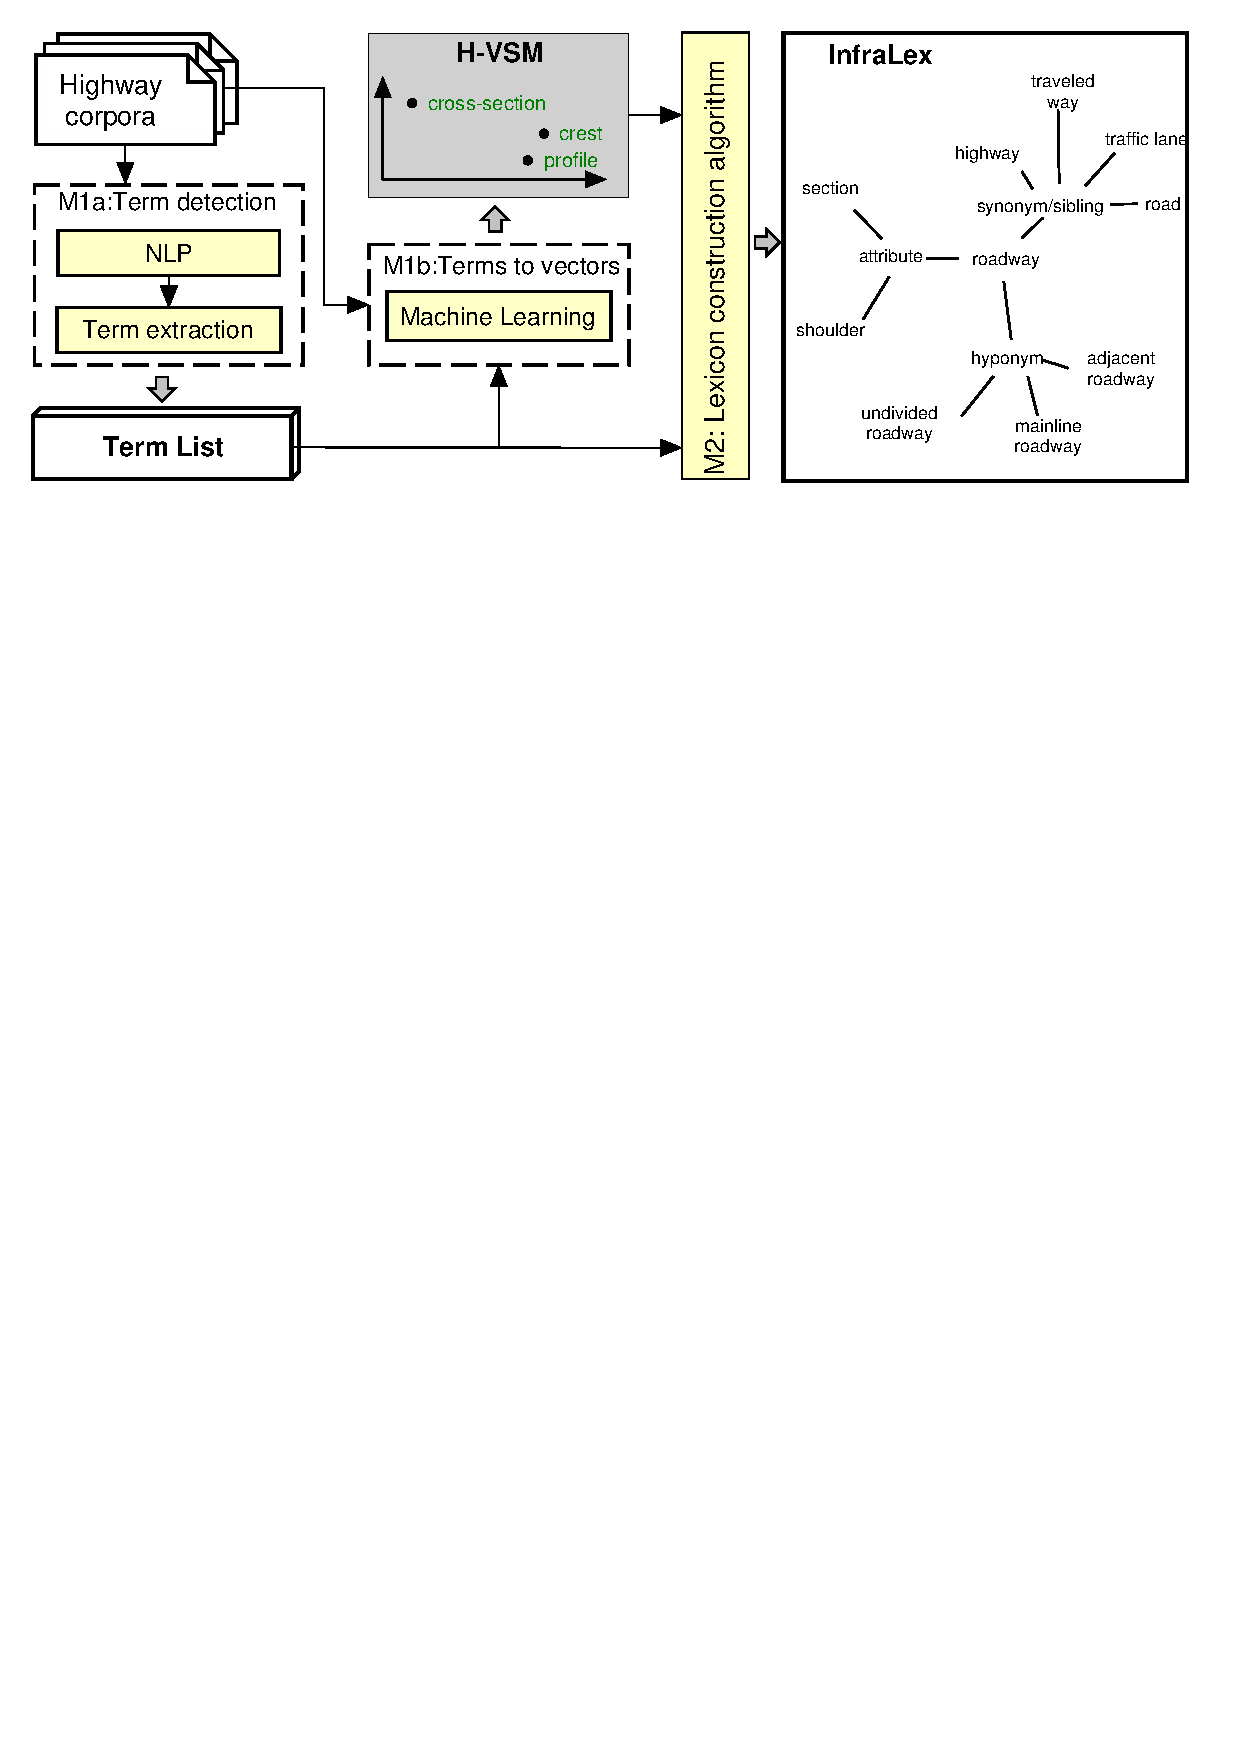
\includegraphics[width=0.95\textwidth]{Figure1_overview_methodology}
	\caption{Overview of the proposed methodology}
	\label{fig:framework}
\end{figure}
%
The ultimate goal of this research is to construct a machine-readable dictionary of technical terms, named InfraLex, for the infrastructure sector. Figure \ref{fig:framework} presents an overview of the methodology proposed to develop InfraLex. The research framework consists of two major modules that are to: (1) train a highway vector space model (H-VSM), and (2) develop an algorithm integrating H-VSM and various linguistic patterns to construct InfraLex. The first module implements several basic NLP techniques (including tokenizing, POS tagging, etc.) and C-value method \cite{frantzi20} to extract highway related technical terms from a highway corpora. The Skip-gram model, an unsupervised machine learning platform proposed by \citeN{mikolov13a}, is then employed to train the semantic similarity between technical terms. The model uses the unlabeled highway corpora as the training dataset. This training process transforms the identified terms into representation vectors in a coordinate space model named H-VSM.  Using this term vector space, the similarity degree between technical terms can be determined; and based on that the list of nearest terms for a given term can be obtained. The second module designs an algorithm for identifying the relation (e.g., synonymy, hypernymy, hyponymy, or attribute) between each item in the nearest list and the target term. The InfraLex lexicon is finally constructed by organizing the domain vocabulary into a network of terms which link to each other through the identified semantic relations. Specifically, the procedure followed to compile the InfraLex dictionary is comprised of the following steps: (a) collect highway technical documents to compose a domain corpus; (b) extract the multi-word terms from the highway corpus; (c) prepare the training dataset for training the H-VSM model; (d) select appropriate values for the training parameters and perform the training of the H-VSM model; and (e) design an algorithm to classify related terms into groups of lexical relations. The below sections discuss these steps in detail.
%\begin{enumerate} [label=(\alph*)]
%\item 
%\item 
%\item 
%\item 
%\item 
%\end{enumerate}
%
%TODO: The preliminary result is presented by. In this paper, the model is extended with larger training datasets and post-processing to reorganize terms in categories which improves the semantic data searching algorithm.
%\section{Highway term space model development} \label{sec:vector-space}
%
%introduction to the distributional vector model, fundamental theory,  the overall process to translate technical terms into vectors representations. the role of vector space allow measure the similarity between 
%TODO: This section presents the extension of the H-VSM developed by the authors' previous work with the extending of training datasets and post-processing of the vector space model.
%
\subsection{Data collection}
%how to collect data, how to clean data to get them readay for training model
%aim text folow remained, flow direction. bottom down, 
%remove heading (chapter, section, subsection), footnote, numerbing, bullets, hyperlink, url, 
As mentioned earlier, H-VSM was trained using a machine learning model which requires a text corpus as the source of the training dataset. The input text corpus was built upon a plethora of highway engineering manuals from the Federal Department of Transportation (DOT) and from 22 State DOTs. The technical terms in a guidance document in the engineering field are organized in various formats such as plain text, tables, and equations. Since tables and equations are not yet supported by the state-of-the-art NLP techniques, they were removed from the text corpus. The final outcome of this phase is a plain text corpus consisting of 16 million words. This dataset is utilized to extract highway related technical terms which are then trained and converted into representation vectors.
%
\subsection{Multi-word terms extraction}
%
\begin{figure}[t]
	\centering
	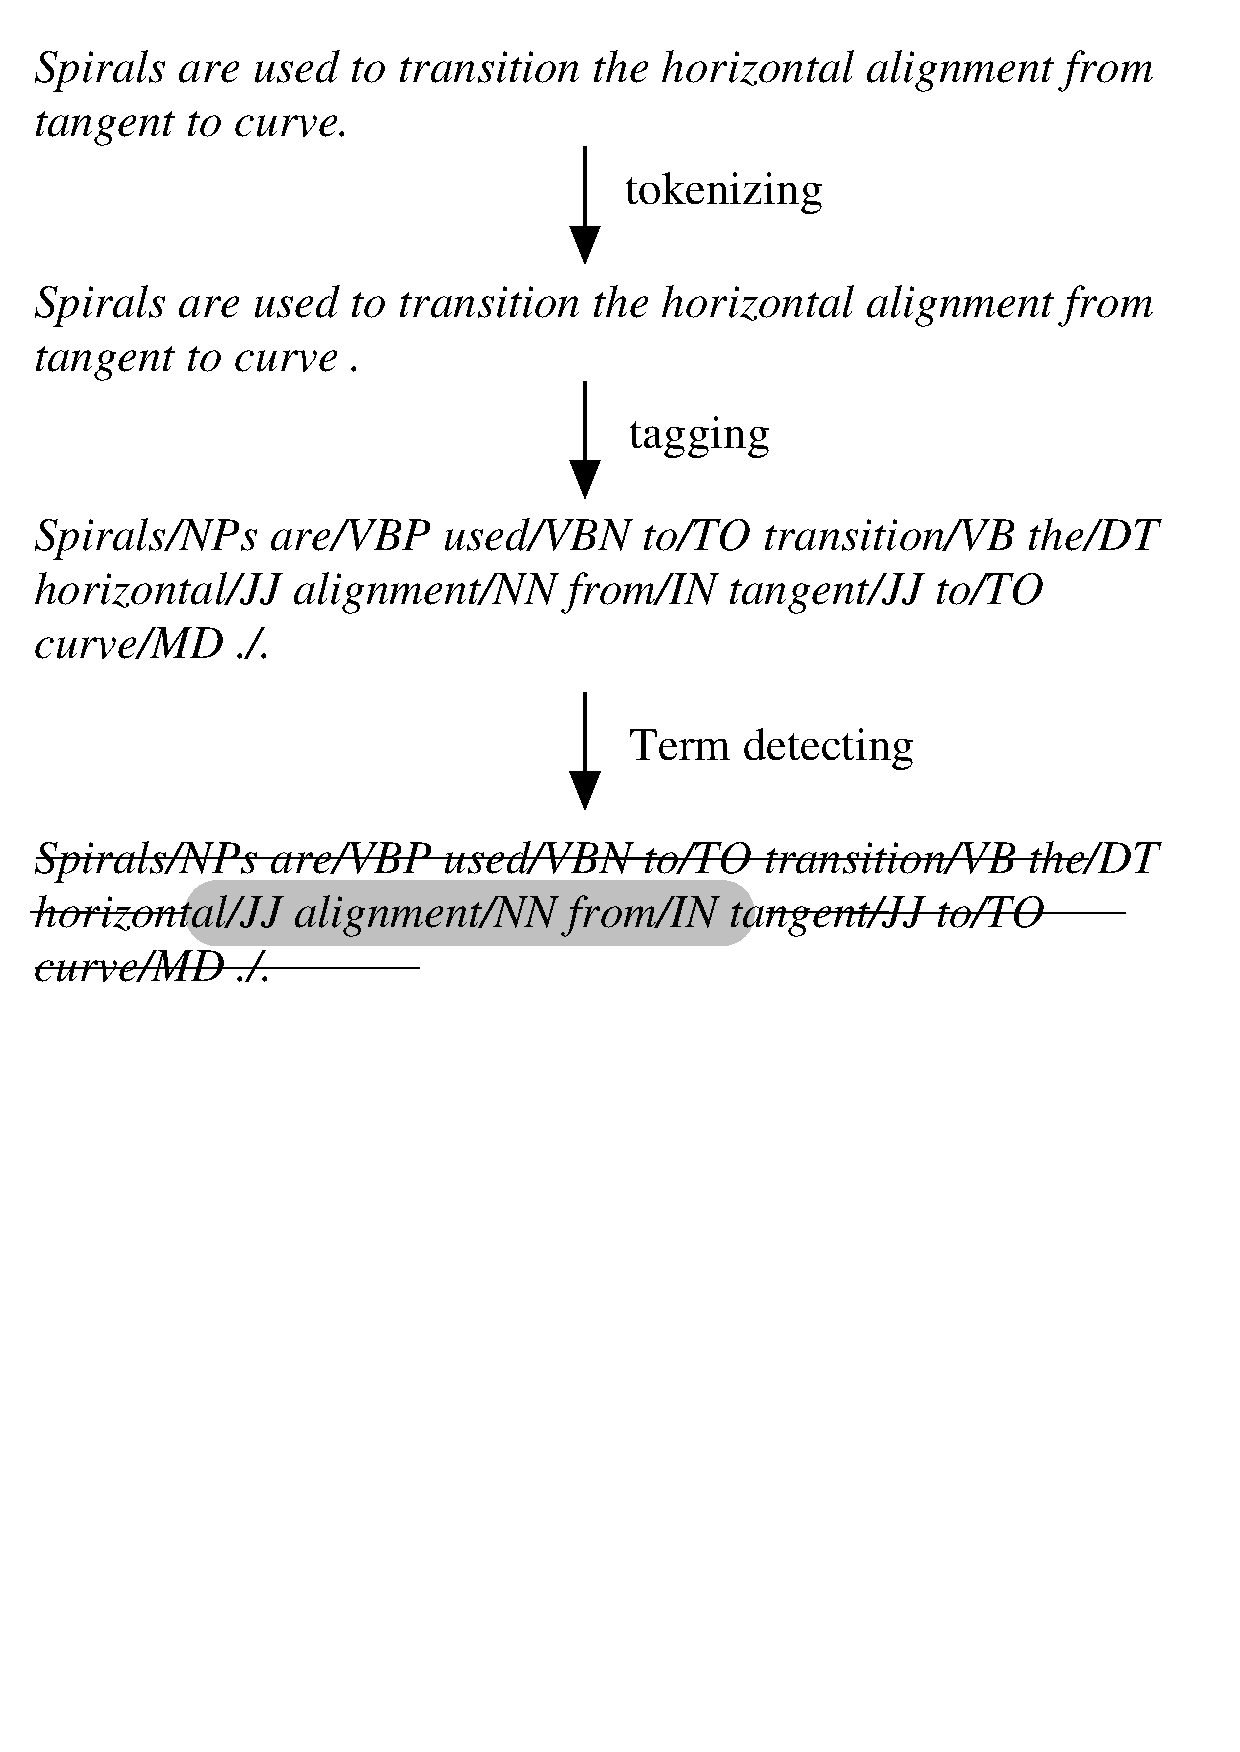
\includegraphics[width=0.45\textwidth]{Figure2_term_extraction}
	\caption{Linguistic processing procedure to detect technical terms}
	\label{fig:np_detect}
\end{figure}
%
A technical term can be a single word (e.g., roadway, lane, etc.) or be composed of multiple words (e.g., right of way, at grade intersection, etc.). The meaning of multi-word terms may not be directly interpreted from the meanings of their single words. In order for the Skip-gram model to learn the semantics of multi-word terms, every occurrence of multi-word terms in the corpus needs to be detected and replaced with connected blocks of word members so that they can be treated as single words. Figure \ref{fig:np_detect} presents the process of detecting technical terms from the set of highway technical documents. The process includes the following steps. 
\par
\begin{enumerate} [label=\roman*]
	\item \textbf{Word tokenizing:} In this step, the text corpus is broken down into individual units (also called tokens) using OpenNLP Tokenizer.
	\item \textbf{Part of Speed (POS) tagging:} The purpose of this step is to determine the POS tag (e.g., noun, adjective, verb, etc.) for each token. The OpenNLP package is also utilized for this task. 
	\item \textbf{Noun phrase detection:} Linguists argue that a technical term is either a noun (e.g., road) or a noun phrase (NP) (e.g., right of way) that frequently occurs in domain text documents \cite{justeson95}. Thus, NPs are good multi-word term candidates. Table \ref{table:term_filter} presents the proposed extraction patterns which are modified from the filters suggested by \citeN{justeson95} to extract NPs. %The first two filters directly detect NPs that occur separately, and the third filter is to count for cases where multiple terms are written in conjunctions (e.g., "vertical and horizontal alignment"). To extract NPs from a conjunction, an extra processing is applied to break it into individual NPs. For example, the conjunction 'vertical and horizontal alignment' will become 'vertical alignment' and 'horizontal alignment'. This division process determines the main part ('alignment') which is shared by two NPs and the dependent parts ('vertical' and 'horizontal'). This research uses Stanford Dependencies Parsing tool, which is able to analyze dependencies between sentiment units, to split conjunctions into separate phrases. 
	%
	In addition, in order to avoid the differentiation between syntactic variants of the same term, for example `roadway' and `roadways', term variants need to be normalized. The following are two types of syntactic variants and the proposed normalization methods.
	\begin{table} [t]
		\caption{Term candidate filters}
		\label{table:term_filter}
		\centering
		\small
		\renewcommand{\arraystretch}{1.25}
		\begin{tabular}{l l}
			\hline
			\textbf{Pattern} & \textbf{Examples}\\
			\hline
			(Adj|N)*N		& road, roadway shoulder, vertical alignment\\
			(Adj|N)*N Prep (of/in) (Adj|N)*N	&	right of way, type of roadway\\
			%(Adj|N)* 'and/or' (Adj|N)*N & vertical and horizontal alignment\\
			\hline
			\multicolumn{2}{l}{\textit{Note:} |, * respectively denote `and/or', and `zero or more'.  } \\
			\hline
		\end{tabular}
		\normalsize
	\end{table}
	%
	\begin{itemize}
		\item \textbf{Type 1} - Plural forms, for example `roadways' and `roadway'. The Porter stemming algorithm \cite{porter80}, which can allow for automated removal of suffixes, is applied on the corpus before extracting NPs.
		\item \textbf{Type 2} - Preposition noun phrases, for example `roadway type' and `type of roadway'. In order to normalize this type of variant, the form with preposition is converted into the non-preposition form by removing the preposition and reversing the order of the remaining portions. For instance, `type of roadway' will become `roadway type'.
		%\item \textbf{Type 3} - Abbreviations, such as AADT. A linguistic rule-based method suggested by \cite{nenadic02} will be used to determine the full NP of an abbreviation. This method suggests the following abbreviation definition patterns: (1) left definition pattern - NP (Abbreviation), for example Annual Average Daily Traffic (AADT); and (2) right definition pattern - (Abbreviation) NP, for example (AADT) Annual Average Daily Traffic.
	\end{itemize}
	\item \textbf{Multi-word term candidate ranking and selection:} Multi-word term definition varies between authors, and there is a lack of formal and widely accepted rules to define if a NP is a multi-word term \cite{frantzi20}. There are a number of methods proposed for estimating termhood (the degree that a linguistic unit is a domain-technical concept), such as TF-IDF  \cite{sparck72,salton88}, C-Value \cite{frantzi20}, Termex  \cite{sclano07}. These methods are based on the occurrence frequencies of NPs in the corpus. Among these methods, Termex outperformed other methods on the Wikipedia corpus, and C-Value was the best on the GENIA medical corpus \cite{zhang08}. This result indicates that the C-value method is more suitable for term extraction from a domain corpus rather than a generic corpus. For this reason, the C-value has been widely used to extract domain terms in the biomedical field, for instance studies performed by \citeN{ananiadou20}, \citeN{lossio13}, and \citeN{nenadic02}. Since the corpus used in this study was mainly collected from technical domain documents, C-value would be the most suitable for the termhood determination task. The C-value measure, as formulated in Equation \ref{eq:cvalue}, suggests that the longer a NP is, the more likely that is a term; and the more frequently it appears in the domain corpus, the more likely it will be a domain term.
	% 
	\begin{equation}
	C-value(a)=
	\begin{cases}
	log_2|a|.f(a), & \text{if a is not nested} \\
	log_2|a|(f(a)-\frac{1}{P(T_a)}\sum_{b\in T_a} f(b)), & \text{otherwise}
	\end{cases}
	\label{eq:cvalue}
	\end{equation}
	%
	Where:
	\begin{description}
		\item[a] is a candidate noun phrase
		\item[|a|] is the length of noun phrase \textit{a}
		\item[f] is the frequency of \textit{a} in the corpus
		\item[Ta] is the set of extracted noun phrases that contains \textit{a}
		\item[P(Ta)] is the number of these candidate terms.
	\end{description}
\end{enumerate}
%
\par
The term extraction process above results in a dataset containing the detected terms along with their termhood scores. These terms are ordered by C-value, and the ones that have negative C-values are discarded. 
\par
To remove non-terms from the term candidate list, a manual evaluation process is conducted. Table \ref{table:term_evaluation} illustrates the evaluation results for several excerpts of the extracted candidates. Since a longer candidate list requires more evaluation effort, NPs with low occurrence frequencies that are unlikely to be technical terms should be automatically eliminated before the manual evaluation. With the frequency threshold of 2, the list consists of 112,024  terms. The list size drops to 8,922 when a threshold of 50 is used. Manual review of such a long list is still a challenging task. To minimize both laborious work and the number of true terms wrongly discarded, the list was evaluated at several ranges of C-values. The precision values, which represent the percentage of real terms in these groups, are presented in Figure \ref{fig:term_precision}. As shown in the figure, precision values are relatively low for groups with c-values less than 70. To balance between human effort and precision of the final term list, this research applied a manual review on all of the automatically extracted terms below the c-value threshold of 70.
%To calculate the recall value, expert is required to final all true terms from the corpus \cite{frantzi20}. with the large corpus in this research, it is impossible to do this task. 
%
\begin{table} [t]
	\caption{Excerpts of the extracted candidate terms}
	\label{table:term_evaluation}
	\centering
	\small
	\renewcommand{\arraystretch}{1.25}
	\begin{tabular}{l l l}
		\hline
		\textbf{Term} & \textbf{Termhood} & \textbf{real term?}\\
		\hline
		sight distance		& 9435.314 & yes\\
		design speed & 9052.556 & yes \\
		additional information & 1829.0 & no\\
		typical section & 1801.0  & yes\\
		basis of payment & 1762.478 & no\\
		\hline
	\end{tabular}
	
	\normalsize
\end{table}

\begin{figure}[t]
	\centering
	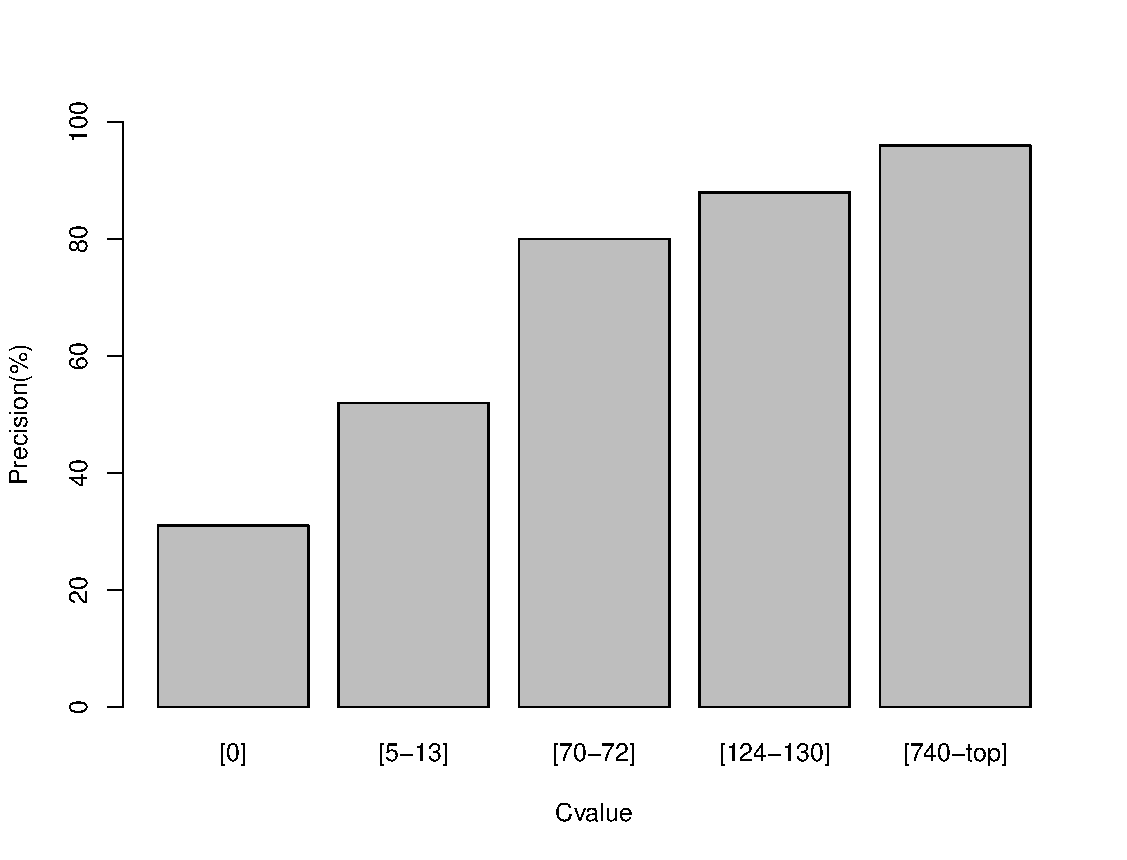
\includegraphics[width=0.5\textwidth]{Figure3_term_precision}
	\caption{Multi-word term extraction evaluation}
	\label{fig:term_precision}
\end{figure}

\subsection{Training dataset preparation}
This step aims at processing the collected text corpus and collecting the training data for developing the H-VSM model. Skip-gram \cite{mikolov13a}, which is an un-supervised machine model, was employed to learn the semantic similarity among words in the text corpus. The Skip-Gram model requires a set of training data in which the input data is a linguistic unit (word or term), and the output data is a set of context words which are closed to the input unit in the corpus. In order to collect this training dataset, the unannotated highway corpus is scanned to capture instances of terms and their corresponding context words. Each occurrence of a word will correspondingly generate a data point in the training dataset.
\par
Before collecting the training dataset, an additional step is needed to handle the issue related to multi-word terms. Since document scanning is on a word-by-word basis, the corpus must be adjusted so that multi-word terms can be treated like single words. To fulfill that requirement, every occurrence of a certain multi-word term in the corpus is replaced with a single unit that is compiled by connecting all the individual words. For instance, `vertical alignment' becomes `vertical-alignment'.
\par
The number of context words to be collected is dependent on the window size that limits how many words to the left and the right of the target word. In the example sentence below, the context of term `roadway' with the window size of 10 will be the following word set \{bike, lane, width, on, a, width, no, curb, gutter\}. Any context word that is in the stop list (the list contains frequent words in English such as `a', `an', and `the' that have little meaning) will be neglected from the context set.
%
\begin{center}
	"The minimum [bike lane width on a \underline{roadway} with no curb and gutter] is 4 feet."
\end{center}
%
\subsection{Semantic similarity training}
%word2vec, brief introduction about word2vec
%skip-gram model
%how to modify the method of selecting conext words
%java program
%
\begin{figure}[t]
	\centering
	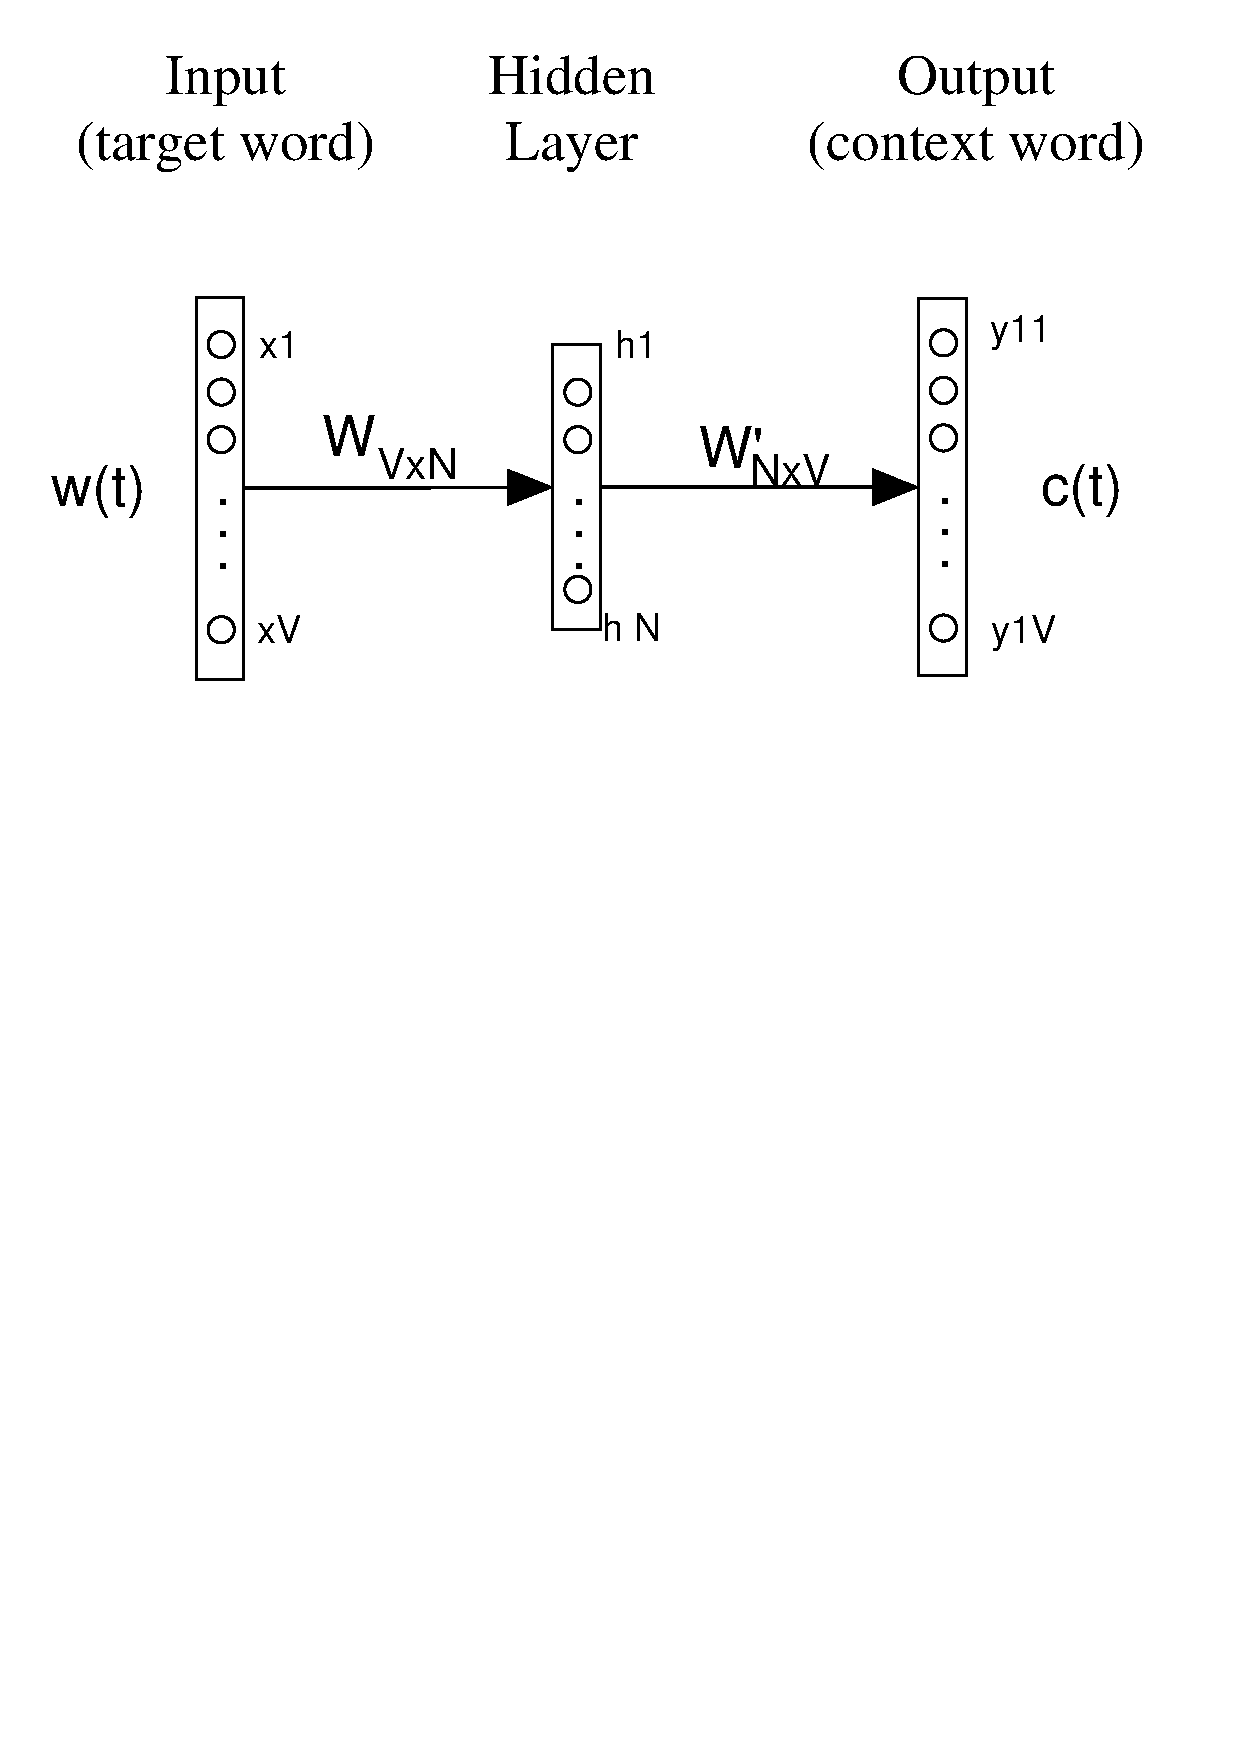
\includegraphics[width=0.45\textwidth]{Figure4_skip-gram-model}
	\caption{Skip-gram model}
	\label{fig:skip-gram}
\end{figure}
%
The semantic similarity is trained using the Word2vec module in the Apache Spark MLlib package \cite{apache16}, an emerging open-source engine, which is based on the Skip-gram neural network model \cite{mikolov13a}. Figure \ref{fig:skip-gram} shows the learning network when the context set includes only one word, where \textit{V} and \textit{N} respectively denote the corpus vocabulary and hidden layer size. In this model, a word is encoded as a one-hot vector of which only the item at the index of the word in the vocabulary is 1, and all other items are 0. The outcome of this machine learning process is a set of term representation vectors  in an N-dimension coordinate system. 
\par
The model includes three major parameters that are \textit{frequency threshold}, \textit{hidden layer size} and \textit{window size} (see Table \ref{table:nn-parameters}). To eliminate those data points with low frequencies of occurrence that are unlikely to be technical terms, Word2vec allows for the use of \textit{frequency threshold}. Any word with the rate lower than the limit will be ignored. \citeN{rehurek14} suggests a range of (0-100) depending on the data set size. Setting this parameter high will enhance the accuracy, but many true technical terms would be out of vocabulary. A preliminary study based on the preliminary corpus with only several millions of words shows that with the frequency of 20, there are very few non-technical terms involved in the training dataset. Hence, with the larger dataset to be collected, this parameter can be higher and up to around 50. The second important parameter is \textit{layer size} which determines the number of nodes in the hidden layer. This parameter highly affects the training accuracy and processing time. A larger layer size is better in terms of accuracy, but this will be paid off by the running time. The reasonable values for this parameter are from ten to hundreds \cite{rehurek14}. The final major parameter, \textit{context window size}, decides how many context words to be considered. Google recommends the size of 10 for the Skip-gram model \cite{google2016}. These parameters are subject to be changed so that the best model can be achieved. The effects of these parameters on the model performance are discussed in Section \ref{sec:eval_infralex}.
%
\begin{table} [t]
	\caption{Skip-gram model parameters}
	\label{table:nn-parameters}
	\centering
	\small
	\renewcommand{\arraystretch}{1.25}
	\begin{tabular}{l l}
		\hline
		\textbf{Parameter} & \textbf{Value}\\
		\hline
		Frequency threshold & 50-100\\
		Hidden layer size		&	100-500\\
		Context window size	&	5,10,15\\
		\hline
	\end{tabular}
	\normalsize
\end{table}
%
\par
Figure \ref{fig:hvsm} presents the term space model of H-VSM derived from the training process when the parameters are set 50, 300 and 10 respectively. H-VSM currently consists of more than 6,000 technical terms. In this model, each technical term is represented as a vector in a high dimensional space. Since the term representation vectors are in a multi-dimensional space; to present the space in 2D graph, PCA (Principle Component Analysis) was used to reduce the size to 2.
\par
The similarity between terms in the H-VSM model can be measured by the angle between two word representation vectors (Equation \ref{equ:cosin_sim}) or the distance between two word points (Equation \ref{equ:dis_sim}). Figure 5 illustrates the clustering of terms by their distances. In this figure, an \textit{inlet} can be inferred to be more similar to an \textit{outlet} (blue) than a \textit{sidewalk} (green). Using this technique, the most similar terms for a given term can be obtained. Table \ref{table:nearest_example} shows a partial ranked list of the nearest terms of `roadway' in order of similarity score.
%
\begin{figure}[t]
	\centering
	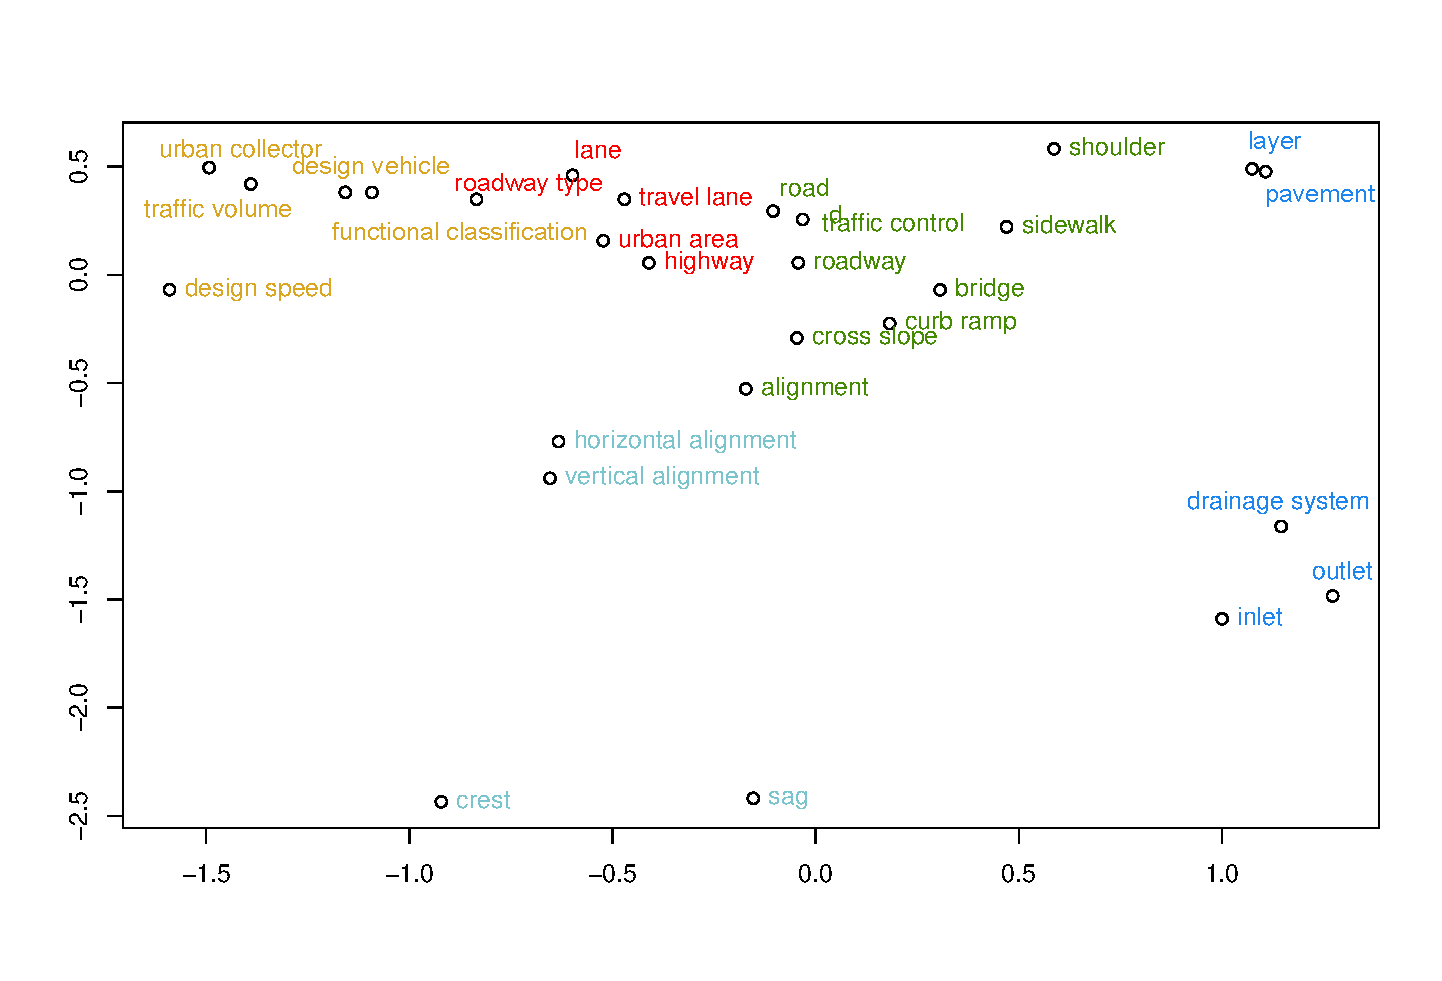
\includegraphics[width=0.95\textwidth]{Figure5_hvsm_space}
	\caption{Highway term space model (H-VSM)}
	\label{fig:hvsm}
\end{figure}
%
\begin{equation}
\label{equ:cosin_sim}
cosine\_similarity = \frac{A.B}{||A||.||B||}
\end{equation}
%
\begin{equation}
\label{equ:dis_sim}
dis\_similarity =\sqrt{(xA_1-xB_1)^2+(xA_2-xB_2)^2+...+(xA_n-xB_n)^2}
\end{equation}

Where: n is the hidden layer size.
%
\begin{table} [t]
	\caption{Examples of top nearest terms}
	\label{table:nearest_example}
	\centering
	\small
	\renewcommand{\arraystretch}{1.25}
	\begin{tabular}{l l l  l}
		\hline
		\textbf{Term} & \textbf{Nearests} & \textbf{Cosine} &\textbf{Rank}\\
		\hline
		roadway			& highway & 0.588 & 1\\
		& traveled-way & 0.583 & 2\\
		& roadway-section & 0.577 & 3\\
		& road & 0.533 & 4\\
		& traffic-lane & 0.524 &5\\
		& separating & 0.522 &6\\
		& adjacent-roadway & 0.519 & 7\\
		& travel-way & 0.517 & 8\\
		& entire-roadway & 0.513 & 9\\
		& ...&...& ...\\
		& roadway-shoulder & 0.505 & 12\\
		& roadway-cross-section & 0.491 & 18\\
		& undivided & 0.452 & 37\\
		& mainline-roadway & 0.450 & 42\\
		\hline
	\end{tabular}
	\normalsize
\end{table}

\subsection{Highway lexicon construction}
The purpose of this module is to construct Infralex, a lexicon of civil engineering technical terms. A lexicon, also known as a lightweight knowledge base, typically includes terms and relations. The core relations of a lexicon are synonym (meaning equivalence), hypernym-hyponym (also known as IS-A or parent-child relation), attribute (concept property), and association (e.g. part-of) \cite{jiang1997semantic,lee13}. Two terms that relate each other through these semantic relations would have a high similarity score. Therefore, the top nearest terms resulted from H-VSM would be a great starting point for detecting relations between technical terms. Table \ref{table:nearest_example} illustrates a list of nearest terms of `roadway'. In this list, the true synonyms are `highway' (1), `traveled-way' (2) and `road' (4); the attributes include `roadway-section' (3), `roadway-shoulder' (12); and `adjacent-roadway' (7) and `undivided' (37) are hyponyms which show different types of roadway.
\par
The specific objective of this task is to detect the semantic relations among terms which are used for rearranging the nearest terms obtained from the H-VSM model. Algorithm \ref{alg:term_class} shows the design pseudo code for classifying the nearest terms of a given target term. The algorithm utilizes linguistic rules and clustering analysis to organize the nearest list into the following three groups: (1) attribute, (2) hyponym, and (3) synonym/sibling. The algorithm, first detects terms belonging to the first two categories using linguistic patterns. The filter rules to detect these relations are presented in Table \ref{table:attribute_pattern}. For a multi-word term matching pattern 1, we can infer that \textit{Noun1} is an attribute of concept \textit{Noun2}; and \textit{Noun2} is an attribute of \textit{Noun1} in the pattern 2. Pattern 3 is for detecting hyponyms where the matched NP is a hyponym of \textit{Noun2} concept.  The remained nearest words will fall into the third group. However, some of them have far or even no relation with the target word. In order to address this issue, this research employed the K-mean clustering algorithm \cite{macqueen67} to split the remained list into three distinct layers based on the similarity score. The terms in the last group are unlikely to be a synonym or sibling; and thus, are removed from the nearest list. The output of the proposed algorithm is a list of classified nearest terms. Table \ref{table:term_clustering} shows one example for the output retrieved from the algorithm. 
%In contrast, since synonym recognition is well known as the process of evaluating the sharing of common attributes, hypernyms, and hyponyms, this process will rely on the results from the detection of other relations. This task will first detect the following relations (hypernyms, hyponyms and attributes) and then use them as features to find synonyms.
%
\begin{algorithm}[h]
	
	\caption{Near term classification algorithm}\label{alg:term_class}
	\begin{algorithmic}[1]
		\State \textbf{Inputs}: term \textit{t}, list of nearest terms \textit{N}, full list of terms \textit{F}
		\State \textbf{Output:}: Classified list of terms \textit{C}
		\Procedure{Term classification procedure}{}
		%\State $\textit{n} \gets \text{size of }\textit{W}$
		%\State $\textit{m} \gets \text{size of }\textit{T}$
		\State $\textit{Att} \gets \text{list of attributes}$
		\State $\textit{Hyp} \gets \text{list of hyponyms}$
		\State $\textit{Syn} \gets \text{list of synonyms}$
		\State $\textit{w} \gets \textit{null}$
		\ForAll {$n \in N$}
		\If {$n$ contains \textit{t}}
		\State $w \gets n$
		
		\Else
		\ForAll {$f \in F$}
		\If {$f$ contains both $n$ and \textit{t}}
		\State $w \gets f$	
		\State Break for
		
		\EndIf
		\EndFor
		\EndIf
		
		\If {$w$ matches \textit{Attribute pattern}}
		\State add $w$ to \textit{Att}
		\ElsIf {$w$ matches \textit{Hyponym pattern}}
		\State add $w$ to \textit{Hyp}
		\Else
		\State add $w$ to \textit{Syn}
		\EndIf
		\EndFor
		\State Cluster \textit{Syn} and discard low relevant terms
		
		\EndProcedure
	\end{algorithmic}
\end{algorithm}
%
%\subsection{Attribute and hyponym patterns}
%
\begin{table} [t]
	\caption{Patterns to extract attributes and hyponyms}
	\label{table:attribute_pattern}
	\centering
	\small
	\renewcommand{\arraystretch}{1.25}
	\begin{tabular}{l l l}
		\hline
		\textbf{Relation} & \textbf{Pattern} & \textbf{Example}\\
		\hline
		Attribute &	Noun1 of Noun2 & the width of the road\\
		& Noun1 Noun2	&	road width, project cost\\
		Hypernym-hyponym & Noun1 Noun2 & vertical alignment isA alignment\\
		\hline
	\end{tabular}
	\normalsize
\end{table}
%
%After the candidate list is refined, the frequency of occurrence for each candidate will then be used to compute the degree that term 'a' is an attribute of concept 'c'. If 'a' is a typical attribute of 'c', it should frequently occur in the corpus. Each concept 'c' will correspondingly have a list of attribute candidates (called list A) and their frequency of occurrences. The likelihood that 'a' is an attribute of concept 'c' is estimated using the normalized probability formula (see Equation \ref{eq:attribute}). The attribute candidates for each concept will be ranked by the likelihood measure and the top list over a threshold value will be accepted as typical attributes. 
%\begin{equation}
%P(a|c)=\frac{n(c,a)}{\sum_{a* \in A} n(c,a)}
%\label{eq:attribute}
%\end{equation}
%\subsection{Synonym/sibling and functional relation recognition}

%
\begin{table} [t]
	\caption{An example in InfraLex}
	\label{table:term_clustering}
	\centering
	\small
	\renewcommand{\arraystretch}{1.25}
	\begin{tabular}{l l l l l}
		\hline
		\textbf{Term}	&\textbf{Relation Group}	& \textbf{Nearests} & \textbf{Cosine} & \textbf{Rank}\\
		roadway			&Synonym					& highway & 0.588 & 1\\
		&							& traveled-way & 0.583 & 2\\
		&							& road & 0.533 & 4\\						
		&							& traffic-lane & 0.524 &5\\ 						
		&							& travel-way & 0.517 & 8\\  \cmidrule{2-5}
		&Attribute					& separating & 0.522 &6\\
		&							& roadway-section & 0.577 & 3\\						
		&							& roadway-shoulder & 0.505 & 12\\
		&							& roadway-cross-section & 0.491 & 18\\\cmidrule{2-5}						
		&Hyponym					& adjacent-roadway & 0.519 & 7\\
		&							& entire-roadway & 0.513 & 9\\
		&							& undivided & 0.452 & 37\\
		&							& mainline-roadway & 0.450 & 42\\
		\hline
	\end{tabular}
	\normalsize
\end{table}


\section{Performance evaluation} \label{sec:eval_infralex}
%evaluation method
This section presents a performance evaluation of InfraLex on the ability to identify synonyms. In this experiment, a gold standard  is used. The gold standard consists of 70 sets of synonyms (both single and multi-word terms) which were examined and extracted from a Wikipedia transportation glossary \cite{wikipedia16}. The developed Infralex model was employed to find the synonym for a given input term. The automatically identified synonym is the nearest word in the synonym/sibling lexical group. The evaluation outcome returns ``true'' if the automatically identified synonym belongs to the actual synonym set of the tested term in the golden standard. The performance was evaluated using the following three measures including precision, recall, and f-measure. Precision refers the accuracy in the conclusions made by the system, and recall reflects the coverage of domain terms of the system. The F score, which is a combined measure of precision and recall, presents the overall performance of a system. 
%
\begin{align} 
&Precision = \frac{\text{number of correctly detected synonyms}}{\text{total detected terms}}  \\
&Recall = \frac{\text{number of correctly detected synonyms}}{\text{total terms}}  \\ 
&F-measure = \frac{2.Precision.Recall}{Precision+Recall}
\end{align}
%results
\begin{table} [b] 
	\caption{Effects of training parameters on performance of synonym matching}
	\label{table:eval_syn_par_effect}
	\centering
	\small
	\renewcommand{\arraystretch}{1.25}
	\begin{tabular}{l l l l l }
		\hline
		\hline
		\textbf{Parameter} & \textbf{Model} & \textbf{Precision (\%)}  & \textbf{Recall(\%)} & \textbf{F (\%)}\\
		\hline
		Baseline	&	50-100-5	&79		&53		&63\\
		\hline
		\textbf{Window size}	&\textbf{50-100-\underline{10}}	&\textbf{81}		&\textbf{54}		&\textbf{65}\\
		&50-100-\underline{15}	&81		&54		&65\\
		\hline		
		Frequency threshold	&\underline{75}-100-5	&74		&50		&60\\
		&\underline{100}-100-5	&77		&51		&62\\
		\hline
		Hidden layer size	&50-\underline{200}-5	&79		&53		&63\\
		\hline
		\hline
	\end{tabular}
	\normalsize
\end{table}
%
%synonym matching peformance result
Table \ref{table:eval_syn_par_effect} shows the performance with various training model settings. The parameters of the baseline model are 50, 100 and 5 respectively for frequency threshold, hidden layer and window size. The authors changed these parameters one by one and kept the other ones unchanged to evaluate their effects to the model performance. As presented in the table, the increase of window size to 10 or 15 resulted in the best model which has a precision of 81\% and an F-measure of 65\%. The change of other parameters did not improve the performance. Especially, the increase of frequency threshold value has negative impact. 
%compared to the previous publication by the authors, this algorithm has been improved with significantly higher accuracy. the post-processing is one reason for the out-performance of the proposed method.  
%
%result
\begin{table} [b] 
	\caption{Comparison of synonym matching performance between Wordnet and InfraLex}
	\label{table:eval_syn_vs_Wordnet}
	\centering
	\small
	\renewcommand{\arraystretch}{1.25}
	\begin{tabular}{l l l l }
		\hline
		\hline
		\textbf{Lexicon} & \textbf{Precision (\%)}  & \textbf{Recall(\%)} & \textbf{F (\%)}\\
		\hline
		Wordnet	&76 	&40 	&52\\	
		\textbf{InfraLex} &\textbf{81}	&\textbf{54}		&\textbf{65}\\	
		\hline
		\hline
	\end{tabular}
	\normalsize
\end{table}
\par
The proposed model was also compared with the generic Wordnet database. Table \ref{table:eval_syn_vs_Wordnet} presents the comparison of performance between InfraLex (with the 50-100-10 setting) and Wordnet. As shown, InfraLex outperforms Wordnet in all measures, and the combined F-measure is significantly improved (65\% compared to 52\%). The biggest contribution to the improvement of the overall F-measure is the recall value which represents a better coverage of domain vocabulary of InfraLex. 
%attribute  hyponyms and attributes. finding performance
%for attribute and hyponym only precision is determined. to determine the recall require of all possible true attributes for a concept which is challenging and unrealistic task, this research evaluate the accuracy of the extracted attributes. this largely depend on the size and the variety of discipiline covered in the corpus. select of one in each set of synonyms in the gold standard and  humam evaluate attribute and non-attribute. the performance in measure using Equation which represent the percentage of correctly extracted attribute/hyponym. 

%
\section{Discussions} \label{sec:dis}
%potential application
This research contributes the body of knowledge in digital exchange of life-cycle project data by developing a lexicon which can serve as a machine-readable dictionary of the domain technical terms. InfraLex is expected to become a fundamental resource that can be applied not only to address the issue of semantic interoperability but also to enhance data query systems and to support natural language processing in the civil infrastructure domain. For example, the developed InfraLex lexicon can eliminate the mismatch of data labels when integrating data from various states to develop a national database (e.g., unit cost, productivity, road condition, etc.). Also, questionnaire designers can utilize InfraLex to search for synonyms so that appropriate terms can be selected for specific groups of potential respondents who might be from multiple disciplines or regions. Furthermore, the query systems for extracting data from digital models would be able to find alternative ways to query data when users' keywords do not match any entity in the database. Since users have different ways and keywords to query data, the ability to recognize synonyms and related concepts of a query system would provide flexibility to the end user. In addition to the applications relevant to data representation discrepancy, this research also have a broad impact to the NLP related research. NLP based platforms can utilize this resource for term sense analysis which is crucial for text mining to extract meaningful information from text documents. Information retrieval systems can also use the semantic relations provided by InfraLex to extract relevant project documents by analyzing the the relatedness between the user's input and the keywords in the documents. By allowing computer systems to understand technical terms which are a basic unit of human language, this study is also expected to fundamentally transform the way human interacts with machine.
\par
%
%limitation and potential direction for improvement
The current study has some limitations that may contribute the low overall performance. First, the highway corpus is still relatively small with only 16 million words, compared to the corpus sizes in other domains with billions of words. Since the recall value largely depends on the corpus size, the expansion of the highway corpus would enable more technical terms to be covered in InfraLex. Future research is needed to enhance the performance of InfraLex by enlarging the data training set in both size and the number of disciplines involved throughout the life cycle of a highway project, such as asset management, project programming, construction management. The corpus also needs to cover other types of transportation assets like bridge, tunnel, railway, culvert, etc. Another work that can potentially improve the model performance is to distinguish synonym and sibling which are still in the same group in the InfraLex system. When these two lexical relations are separated, the possibility of recognizing a wrong synonym will be reduced; and consequently, the precision value would be enhanced.
\section{Conclusions} \label{sec:conclns3} 
Data manipulation from multiple sources is a challenging task in infrastructure management due to the inconsistency of data format and terminology. The contribution of this study is a digital lexicon of highway related technical terms (named InfraLex) which can enable a computer to understand semantic meanings of terms.  This research employs advanced NLP techniques to extract technical terms from a highway text corpus which is composed of 16 million words built on a collection of design manuals from 22 State DOTs across the U.S. Machine learning was used to train the semantic similarity between technical terms. An algorithm was designed to classify the nearest terms resulted from the semantic similarity model into distinct groups according to their lexical relationships. This algorithm was employed to develop the InfraLex database. 
\par
The developed lexicon has been evaluated by comparing the results obtained from the computational model and a man-crafted gold standard. The result shows an accuracy of over 80 percent.  The best model is associated with the training parameters of 50, 100 and 10 respectively for frequency threshold, hidden layer size, and window size. Although significant improvement is shown in comparison with the existing thesaurus databases, the overall performance is not relatively high. This might be due to the size of the training data. Future research will be conducted to expand the highway corpus to further disciplines such as asset management, and transportation operation. 
\par
The research opens a new gate for computational tools regarding natural language processing in the highway sector. InfraLex would enable computer systems to understand terms and consequently enable the extraction of value information from project documents and transform the way human interacts with computer by allowing users to use natural language. 

\bibliography{mybib}
%
%
\end{document}

